\begin{figure}[tbp]
\centering
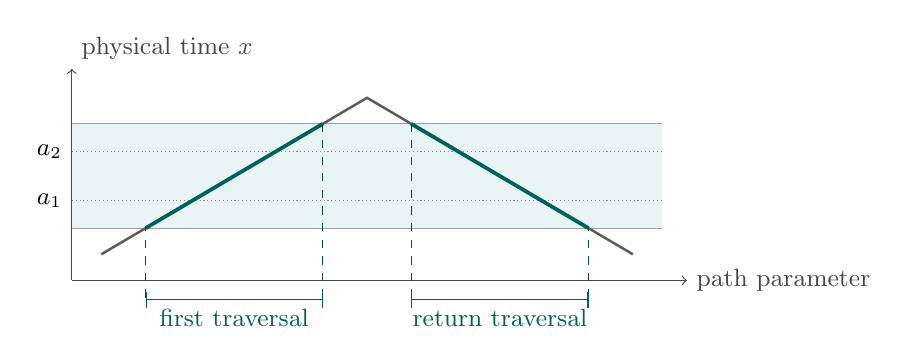
\begin{tikzpicture}[x=1.25cm,y=0.92cm,font=\small]
  \fill[teal!9] (0,0.72) rectangle (6.0,2.16);
  \draw[black!38] (0,0.72)--(6,0.72) (0,2.16)--(6,2.16);
  \foreach \y/\lab in {1.1/{a_1},1.78/{a_2}} {
    \draw[black!46,densely dotted] (0,\y)--(6,\y);
    \node[left] at (0,\y) {$\lab$};
  }
  \draw[->,black!72] (0,0)--(6.25,0) node[right] {path parameter};
  \draw[->,black!72] (0,0)--(0,2.92) node[above right] {physical time $x$};
  \draw[black!64,line width=.9pt] (.3,.36)--(3,2.52)--(5.7,.36);
  \draw[teal!75!black,line width=1.35pt] (.75,.72)--(2.55,2.16);
  \draw[teal!75!black,line width=1.35pt] (3.45,2.16)--(5.25,.72);
  \foreach \x/\y in {.75/.72,2.55/2.16,3.45/2.16,5.25/.72}
    \draw[teal!60!black,dashed] (\x,-.24)--(\x,\y);
  \draw[|-|,teal!75!black] (.75,-.27)--(2.55,-.27)
    node[midway,below] {first traversal};
  \draw[|-|,teal!75!black] (3.45,-.27)--(5.25,-.27)
    node[midway,below] {return traversal};
\end{tikzpicture}
\caption{Two visits to the same physical interval (shaded) occupy disjoint
parts of the path parameter. Each visit incurs a distinct interior break
for each tracer mark $a_1,a_2$. Only the time projection is drawn. A
break in a tracer coordinate need not be visible in that projection.}
\label{fig:return-traversals}
\end{figure}
